\documentclass[border=10pt]{standalone}

\usepackage{tikz}
\usepackage{tikzsymbols}
\usetikzlibrary{calc,patterns,shapes.geometric}

\def\centerarc[#1](#2)(#3:#4:#5){\draw[#1] ($(#2)+({#5*cos(#3)},{#5*sin(#3)})$) arc (#3:#4:#5);}

\begin{document}
	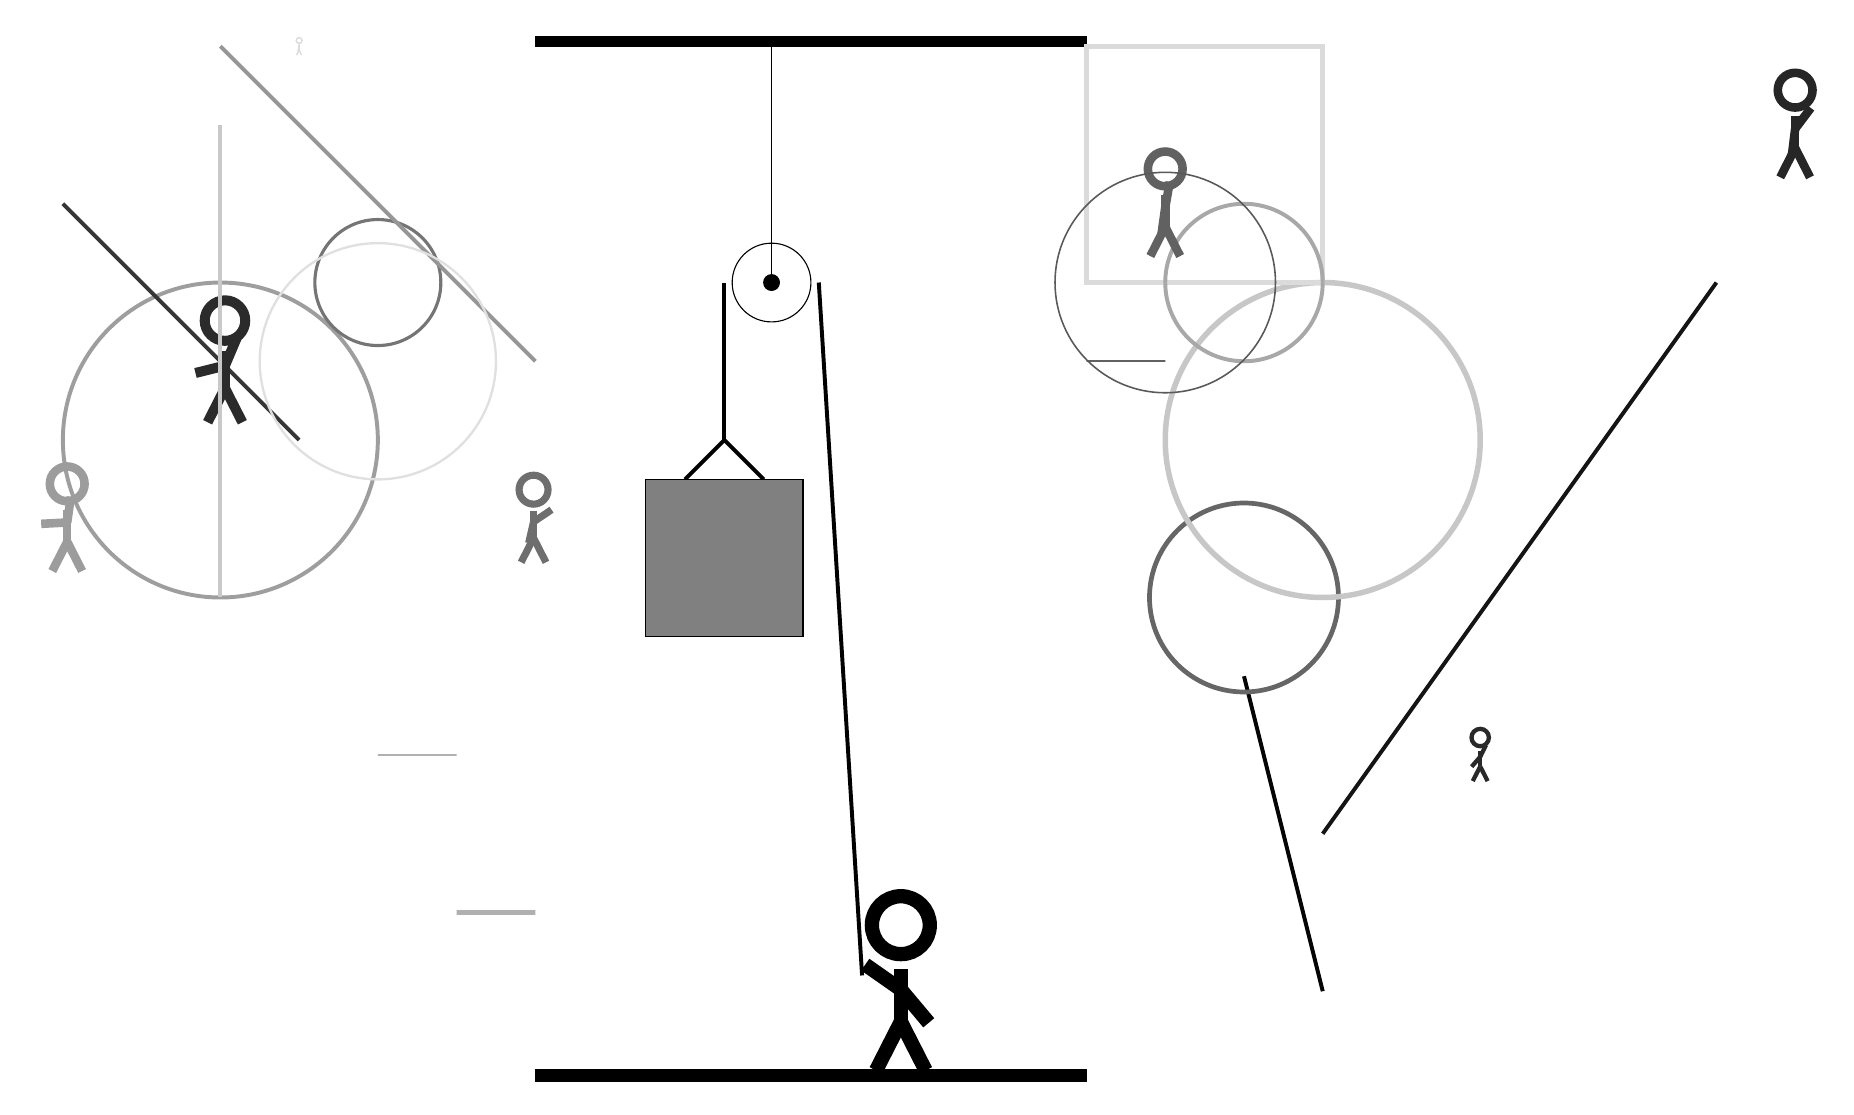
\begin{tikzpicture}
		%%%%% START %%%%%
		
		\draw[fill=black] (-2, 10) rectangle (5, 10.125);
		
		\draw (1, 7) circle (0.5);
		\draw[fill=black] (1, 7) circle (0.1);
		\draw (1, 10) -- (1, 7);
		
		\draw[line width=0.5mm] (-0.1, 4.5) -- (0.4, 5.0) -- (0.9, 4.5);
		\draw[fill=black!50] (-0.6, 4.5) rectangle (1.4, 2.5);
		
		\draw [line width=0.5mm, color=black!38](-6, 5) circle (2.0);
		
		\node[line width=0.2mm, color=black!39] at (-8, 4) {\Strichmaxerl[6][3][82]};
		\draw[line width=0.5mm, color=black!98](8, -2) -- (7, 2);
		\draw[line width=0.5mm, color=black!79](-5, 5) -- (-8, 8);
		\node[line width=0.3mm, color=black!85] at (14, 9) {\Strichmaxerl[6][83][53]};
		\node[line width=0.3mm, color=black!83] at (-6, 6) {\Strichmaxerl[7][14][67]};
		\draw [line width=0.6mm, color=black!60](7, 3) circle (1.2);
		\draw [line width=0.7mm, color=black!22](8, 5) circle (2.0);
		\draw [line width=0.4mm, color=black!54](-4, 7) circle (0.8);
		\draw[line width=0.5mm, color=black!21](-6, 3) -- (-6, 9);
		\node[line width=0.4mm, color=black!14] at (-5, 10) {\Strichmaxerl[1][75][87]};
		
		\draw[line width=0.3mm, color=black!31] (-4, 1) rectangle (-3, 1);
		\draw[line width=0.7mm, color=black!31] (-3, -1) rectangle (-2, -1);
		
		\draw[line width=0.6mm, color=black!14] (5, 7) rectangle (8, 10);
		\draw [line width=0.5mm, color=black!34](7, 7) circle (1.0);
		\draw[line width=0.3mm, color=black!62] (6, 6) rectangle (5, 6);
		
		\node[line width=0.4mm, color=black!84] at (10, 1) {\Strichmaxerl[3][49][64]};
		\draw [line width=0.7mm, color=black!96](-5, 4) circle (0.0);
		\node[line width=0.7mm, color=black!62] at (6, 8) {\Strichmaxerl[6][82][80]};
		\draw [line width=0.2mm, color=black!65](6, 7) circle (1.4);
		\draw[line width=0.5mm, color=black!41](-6, 10) -- (-2, 6);
		\node[line width=0.4mm, color=black!57] at (-2, 4) {\Strichmaxerl[5][77][34]};
		\draw [line width=0.3mm, color=black!12](-4, 6) circle (1.5);
		\draw[line width=0.5mm, color=black!92](8, 0) -- (13, 7);
		
		\draw[line width=0.5mm] (0.4, 7) -- (0.4, 5.0);
		\centerarc[line width=0.5mm](1, 7)(0:180:0.6);
		\draw[line width=0.5mm](1.6, 7) -- (2.15, -1.8);
		
		\node at (2.6, -1.9) {\Strichmaxerl[10][-35][-50]};
		
		\draw[fill=black] (-2, -3) rectangle (5, -3.15);
		
		%%%%% END %%%%%
	\end{tikzpicture}
\end{document}